%% Beispiel-Präsentation
\documentclass[de,16:9]{sdqbeamer} 
 
%% Titelbild
\titleimage{banner_2020_kit}

%% Gruppenlogo
% \grouplogo{SDQ-Logo-new.png} 
\grouplogo{}

%% Gruppenname
% \groupname{Abteilungs-, KIT-Fakultäts-, Institutsbezeichnung}

% Beginn der Präsentation

\title[Optimierungsansätze für Adaptionsstrategien in SAS]{Optimierungsansätze für Adaptionsstrategien in SAS}
\author[Tim Engbrocks]{Tim Engbrocks}

\date[21.\,07.\,2021]{21.\,07.\,2021}

% Literatur 
 
\usepackage[citestyle=numeric,style=numeric,backend=biber]{biblatex}
\addbibresource{presentation.bib}
\bibhang1em

\begin{document}

%Titelseite
\KITtitleframe

%Inhaltsverzeichnis
\begin{frame}{Inhaltsverzeichnis}
\tableofcontents
\end{frame}

\section{Einführung}

\begin{frame}{Die Komplexität von Software}
	\begin{center}
		Die Komplexität von Software steigt stetig. \\
		\glqq The looming software crisis \grqq - IBM, 2001
	\end{center}
	\medskip
	\begin{itemize}
		\item Moderne Sprachmodelle: 
		\begin{itemize}
			\item GPT-3 von OpenAI: 175 Milliarden Parameter \cite{GPT3}
			\item Turing-NLG von Microsoft: 17 Milliarden Parameter \cite{TuringNLG}
		\end{itemize}
		\item Teslas Autopilot AI sagt 10.000 Parameter vorraus \cite{TeslaAutopilot}
	\end{itemize}
\end{frame}

\begin{frame}{Netflix Microservice Architektur}
	\begin{columns}
		\column{.7\textwidth} \begin{center}
			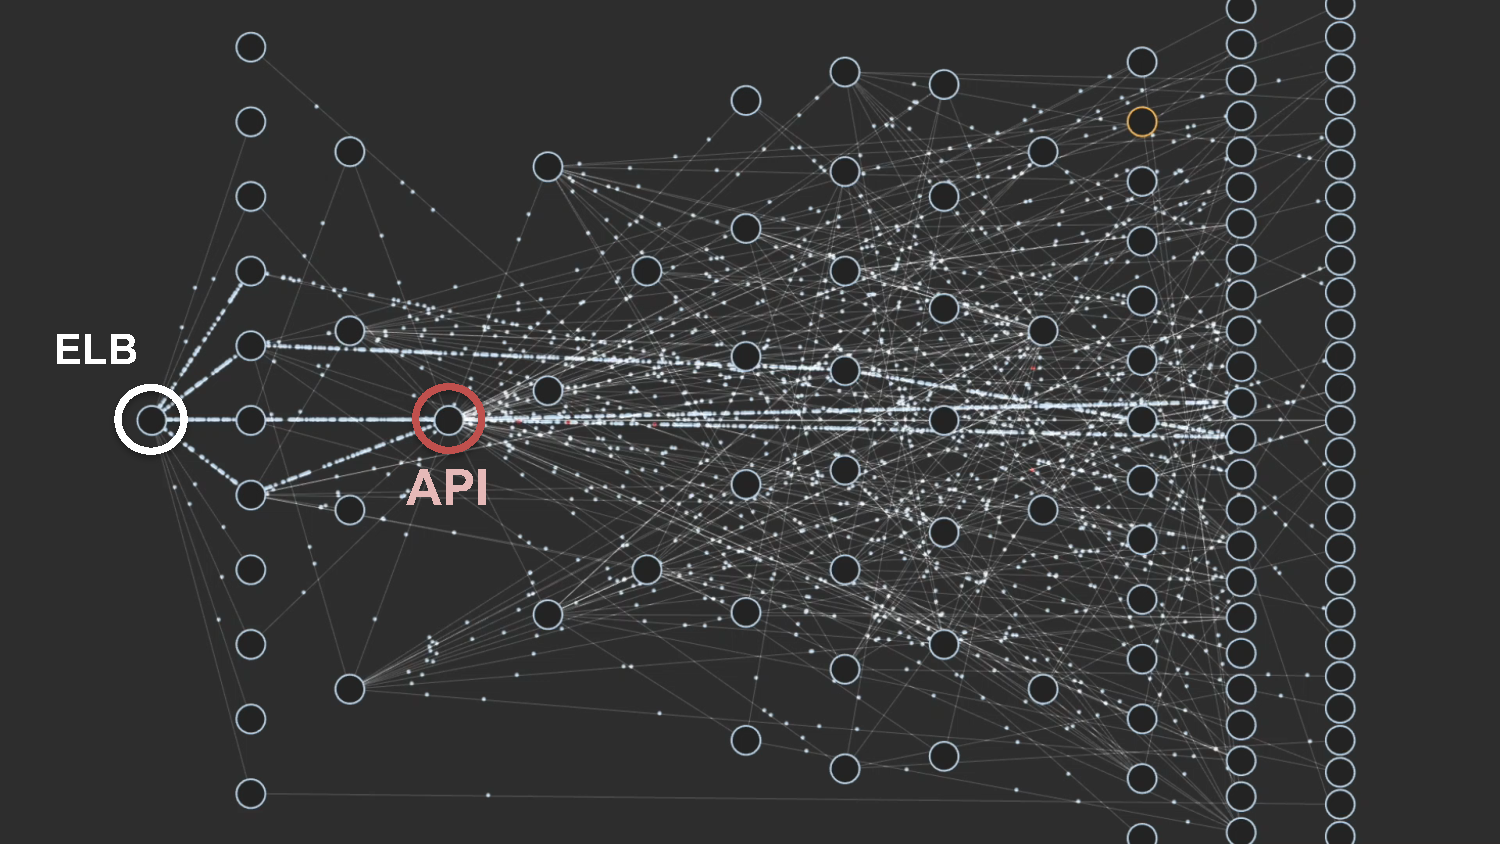
\includegraphics[width=0.9\textwidth]{sources/Mastering Chaos.pdf}
		\end{center}
		\column{.3\textwidth} Josh Evans, CTO @ Netflix, QCon 2016 \cite{JoshQCon}
	\end{columns}
\end{frame}

\begin{frame}{Die Lösung: Autonomes Management}
	\begin{columns}
		\column{.7\textwidth} \begin{center}
			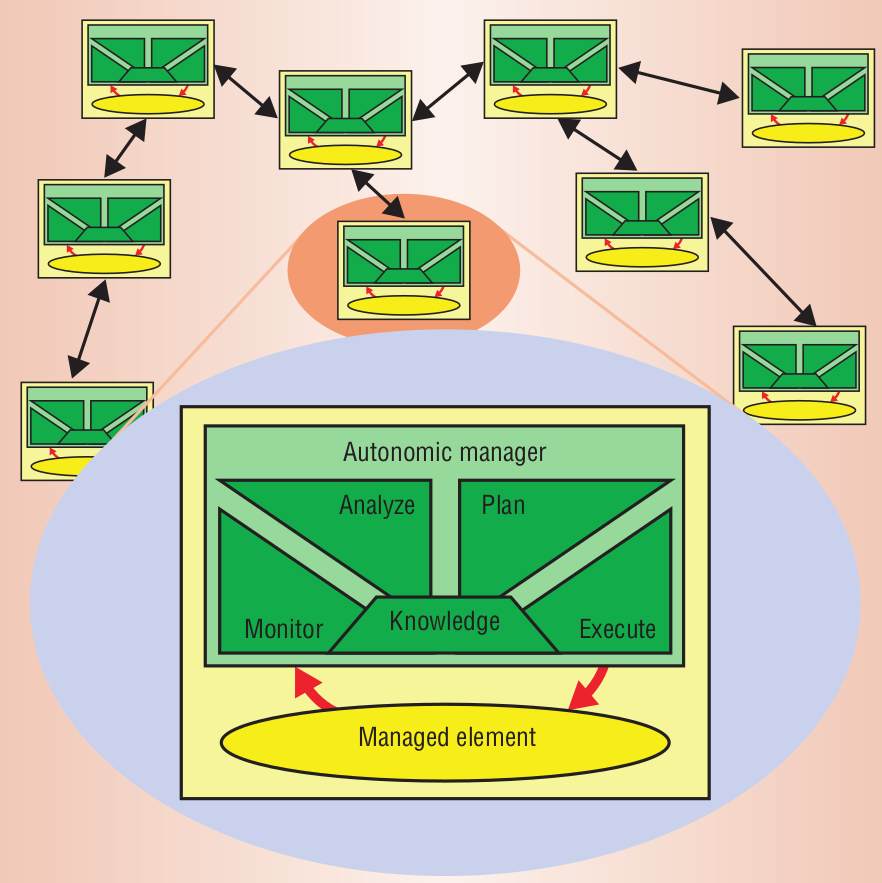
\includegraphics[height=0.7\textheight]{sources/MAPEK.png}
		\end{center}
		\column{.3\textwidth} \cite{VisionOfAutonomicComputing}
	\end{columns}
\end{frame}

\section{Selbstadaptive Systeme}

\begin{frame}{Definition}
	\begin{greenblock}{Selbstadaptives System}
		Ein System, das sich autonom steuert durch das:
		\begin{itemize}
			\item \textit{Beobachten} des Kontextes
			\item \textit{Analysieren} von Veränderungen
			\item \textit{Planen} von Anpassungen
			\item \textit{Ausführen} von Anpassungen
		\end{itemize}
	\end{greenblock}
\end{frame}

\begin{frame}{Beispiel: kommerzielles Web Angebot}
	\begin{itemize}
		\item Szenario: System Administrator eines kommerziellen Web Angebots.
		\item Tägliche Aufgabe: System Paramter X basierend auf Metrik Y anpassen.
	\end{itemize}
	\medskip
	Dieses Szenario kann von einem Selbstadaptiven System profitieren:
	\begin{itemize}
		\item Generelle Anpassungs Regel:
		Wenn die Metrik Y den Schwellwert Z übersteigt: Passe den System Parameter X an
		\item Beispiel: Wenn die Serverlast zu hoch wird: Starte einen zusätzlichen Server
	\end{itemize}
\end{frame}

\begin{frame}{Selbstadaptive Systeme klassifizieren}
	\begin{columns}
		\column{.7\textwidth} \begin{center}
			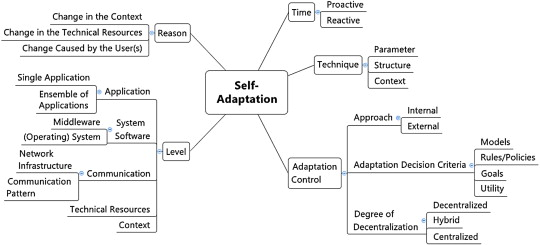
\includegraphics[width=\textwidth]{sources/KrupitzerTaxonomy.jpg}
		\end{center}
		\column{.3\textwidth} \cite{SurveyOnEngineeringApproaches}
	\end{columns}
\end{frame}

\begin{frame}{Grenzen von Selbstadaptiven Systemen}
	\begin{center}
		\Large \textbf{Unsicherheit}
		\\ \medskip
		Änderungen im Kontext $\Rightarrow$ Unerwartete Ergebnisse von Anpassungen
	\end{center}
\end{frame}

\section{Optimierungsansätze}

\begin{frame}{Optimierungen für Selbstadaptive Systeme}
	Der meist verwendete Optimierungsansatz:
	\begin{itemize}
		\item Dynamisch Adaptations Regeln anpassen
	\end{itemize}
	\medskip
	Viele Ansätze verwenden maschinelles lernen, um neue Regeln zu generieren
	oder bestehende anzupassen. \\
	\medskip
	Andere Aspekte des Systems können auch optimiert werden:
	\begin{itemize}
		\item Adaptations Steuerung: Wie
		\item Ebene: Wo
		\item Methode: Was
	\end{itemize}
\end{frame}

\section{Klassifizierung}

\begin{frame}{Eine Klassifizierung entwicklen}
	Die Klassifizierung basiert auf drei Konzepten:
	\begin{itemize}
		\item Reflektive Systeme \cite{FORMS}
		\item Die 6W Fragen \cite{LandscapeAndResearchChallenges}
		\begin{itemize}
			\item Wieso, Wo, Wann, Was, Wer und Wie
		\end{itemize}
		\item Die Klassifizierung von Selbstadaptiven Systemen \cite{SurveyOnEngineeringApproaches}
	\end{itemize}
\end{frame}

\begin{frame}{Vorschlag einer Klassifizierung}
	\begin{center}
		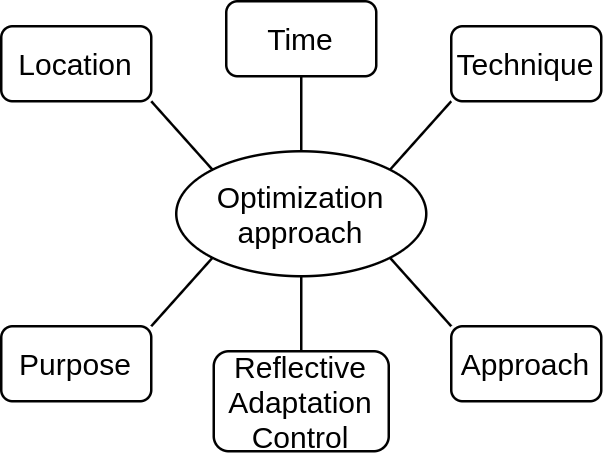
\includegraphics[width=.5\textwidth]{sources/ClassificationProposal-Proposal.png}
	\end{center}
\end{frame}

\begin{frame}{Klassifizierung - Ort}
	\begin{greenblock}{Ort}
		\begin{itemize}
			\item Adaptations Steuerung
			\item Ebene
			\item Methode
		\end{itemize}
	\end{greenblock}
\end{frame}

\begin{frame}{Klassifizierung - Zeit}
	\begin{greenblock}{Zeit}
		\begin{itemize}
			\item Entwurfsphase
			\item Laufzeit / Online Phase
			\item Offline Phase
		\end{itemize}
	\end{greenblock}
\end{frame}

\begin{frame}{Klassifizierung - Methode}
	\begin{greenblock}{Methode}
		\begin{itemize}
			\item Adaptations Regeln
			\item Wissen
			\item Adaptations Methode
			\item Ebene
		\end{itemize}
	\end{greenblock}
\end{frame}

\begin{frame}{Klassifizierung - Zweck}
	\begin{greenblock}{Zweck}
		\begin{itemize}
			\item Vorhandenes Wissen anpassen
			\item Adaptations Regeln an die neue Umgebung anpassen
			\item Ein Ziel erfüllen
			\item Eine Nutzenfunktion maximieren/minimieren
		\end{itemize}
	\end{greenblock}
\end{frame}

\begin{frame}{Klassifizierung - Ansatz}
	\begin{greenblock}{Ansatz}
		\begin{itemize}
			\item Intern / Extern
			\item Grad der Dezentralisierung:
			\begin{itemize}
				\item Komplett zentral
				\item Komplett dezentral
				\item Sowohl zentral als auch dezentral
			\end{itemize}
		\end{itemize}
	\end{greenblock}
\end{frame}

\begin{frame}{Klassifizierung - Reflektive Anpassungs Steuerung}
	\begin{greenblock}{Reflektive Anpassungs Steuerung}
		\begin{itemize}
			\item Modelle anpassen
			\item Adaptations Regeln anpassen
			\item Ziele erfüllen
			\item Nutzenfunktionen maximieren/minimieren
		\end{itemize}
	\end{greenblock}
\end{frame}

\begin{frame}{Vorschlag einer Klassifizierung}
	\begin{center}
		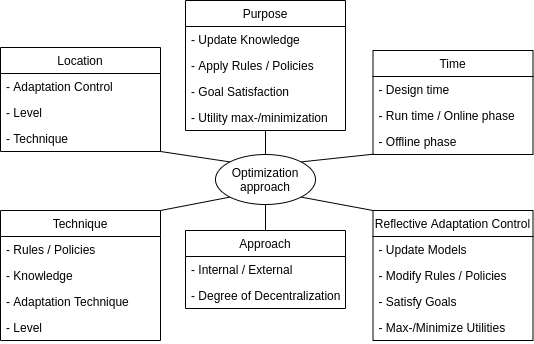
\includegraphics[width=.6\textwidth]{sources/ClassificationProposal-WithDimensions.png}
	\end{center}
\end{frame}

\section{Fazit}

\begin{frame}{Schlussfolgerungen}
	Nur wenige Optimierungsansätze verwenden:
	\begin{itemize}
		\item Zeit: Entwurfsphase und Offline Phase
		\item Ort: Ebene und Technik
		\item Ansatz: Dezentral
	\end{itemize}
\end{frame}

\begin{frame}{Weitere Forschung}
	Folgende Bereiche benötigen weitere Forschung:
	\begin{itemize}
		\item Die vorherigen Dimensionen erforschen
		\item Eine Methode, um den Nutzen von Optimierungsansätzen zu quantifizieren
		\item Selbstadaptive Systeme und Optimierungsansätze, die unabhängig von der Domäne sind
	\end{itemize}
\end{frame}

\appendix
\beginbackup

\begin{frame}{Literatur}
\printbibliography
\end{frame}

%% \section{Farben}
%% ----------------------------------------
%% | Test-Folie mit definierten Farben |
%% ----------------------------------------
% \begin{frame}{Farbpalette}
% \tiny

% % GREEN
% 	\colorbox{kit-green100}{kit-green100}
% 	\colorbox{kit-green90}{kit-green90}
% 	\colorbox{kit-green80}{kit-green80}
% 	\colorbox{kit-green70}{kit-green70}
% 	\colorbox{kit-green60}{kit-green60}
% 	\colorbox{kit-green50}{kit-green50}
% 	\colorbox{kit-green40}{kit-green40}
% 	\colorbox{kit-green30}{kit-green30}
% 	\colorbox{kit-green25}{kit-green25}
% 	\colorbox{kit-green20}{kit-green20}
% 	\colorbox{kit-green15}{kit-green15}
% 	\colorbox{kit-green10}{kit-green10}
% 	\colorbox{kit-green5}{kit-green5}

% % BLUE
% 	\colorbox{kit-blue100}{kit-blue100}
% 	\colorbox{kit-blue90}{kit-blue90}
% 	\colorbox{kit-blue80}{kit-blue80}
% 	\colorbox{kit-blue70}{kit-blue70}
% 	\colorbox{kit-blue60}{kit-blue60}
% 	\colorbox{kit-blue50}{kit-blue50}
% 	\colorbox{kit-blue40}{kit-blue40}
% 	\colorbox{kit-blue30}{kit-blue30}
% 	\colorbox{kit-blue25}{kit-blue25}
% 	\colorbox{kit-blue20}{kit-blue20}
% 	\colorbox{kit-blue15}{kit-blue15}
% 	\colorbox{kit-blue10}{kit-blue10}
% 	\colorbox{kit-blue5}{kit-blue5}

% % RED
% 	\colorbox{kit-red100}{kit-red100}
% 	\colorbox{kit-red90}{kit-red90}
% 	\colorbox{kit-red80}{kit-red80}
% 	\colorbox{kit-red70}{kit-red70}
% 	\colorbox{kit-red60}{kit-red60}
% 	\colorbox{kit-red50}{kit-red50}
% 	\colorbox{kit-red40}{kit-red40}
% 	\colorbox{kit-red30}{kit-red30}
% 	\colorbox{kit-red25}{kit-red25}
% 	\colorbox{kit-red20}{kit-red20}
% 	\colorbox{kit-red15}{kit-red15}
% 	\colorbox{kit-red10}{kit-red10}
% 	\colorbox{kit-red5}{kit-red5}

% % GREY
% 	\colorbox{kit-gray100}{\color{white}kit-gray100}
% 	\colorbox{kit-gray90}{\color{white}kit-gray90}
% 	\colorbox{kit-gray80}{\color{white}kit-gray80}
% 	\colorbox{kit-gray70}{\color{white}kit-gray70}
% 	\colorbox{kit-gray60}{\color{white}kit-gray60}
% 	\colorbox{kit-gray50}{\color{white}kit-gray50}
% 	\colorbox{kit-gray40}{kit-gray40}
% 	\colorbox{kit-gray30}{kit-gray30}
% 	\colorbox{kit-gray25}{kit-gray25}
% 	\colorbox{kit-gray20}{kit-gray20}
% 	\colorbox{kit-gray15}{kit-gray15}
% 	\colorbox{kit-gray10}{kit-gray10}
% 	\colorbox{kit-gray5}{kit-gray5}

% % Orange
% 	\colorbox{kit-orange100}{kit-orange100}
% 	\colorbox{kit-orange90}{kit-orange90}
% 	\colorbox{kit-orange80}{kit-orange80}
% 	\colorbox{kit-orange70}{kit-orange70}
% 	\colorbox{kit-orange60}{kit-orange60}
% 	\colorbox{kit-orange50}{kit-orange50}
% 	\colorbox{kit-orange40}{kit-orange40}
% 	\colorbox{kit-orange30}{kit-orange30}
% 	\colorbox{kit-orange25}{kit-orange25}
% 	\colorbox{kit-orange20}{kit-orange20}
% 	\colorbox{kit-orange15}{kit-orange15}
% 	\colorbox{kit-orange10}{kit-orange10}
% 	\colorbox{kit-orange5}{kit-orange5}

% % lightgreen
% 	\colorbox{kit-lightgreen100}{kit-lightgreen100}
% 	\colorbox{kit-lightgreen90}{kit-lightgreen90}
% 	\colorbox{kit-lightgreen80}{kit-lightgreen80}
% 	\colorbox{kit-lightgreen70}{kit-lightgreen70}
% 	\colorbox{kit-lightgreen60}{kit-lightgreen60}
% 	\colorbox{kit-lightgreen50}{kit-lightgreen50}
% 	\colorbox{kit-lightgreen40}{kit-lightgreen40}
% 	\colorbox{kit-lightgreen30}{kit-lightgreen30}
% 	\colorbox{kit-lightgreen25}{kit-lightgreen25}
% 	\colorbox{kit-lightgreen20}{kit-lightgreen20}
% 	\colorbox{kit-lightgreen15}{kit-lightgreen15}
% 	\colorbox{kit-lightgreen10}{kit-lightgreen10}
% 	\colorbox{kit-lightgreen5}{kit-lightgreen5}

% % Brown
% 	\colorbox{kit-brown100}{kit-brown100}
% 	\colorbox{kit-brown90}{kit-brown90}
% 	\colorbox{kit-brown80}{kit-brown80}
% 	\colorbox{kit-brown70}{kit-brown70}
% 	\colorbox{kit-brown60}{kit-brown60}
% 	\colorbox{kit-brown50}{kit-brown50}
% 	\colorbox{kit-brown40}{kit-brown40}
% 	\colorbox{kit-brown30}{kit-brown30}
% 	\colorbox{kit-brown25}{kit-brown25}
% 	\colorbox{kit-brown20}{kit-brown20}
% 	\colorbox{kit-brown15}{kit-brown15}
% 	\colorbox{kit-brown10}{kit-brown10}
% 	\colorbox{kit-brown5}{kit-brown5}

% % Purple
% 	\colorbox{kit-purple100}{kit-purple100}
% 	\colorbox{kit-purple90}{kit-purple90}
% 	\colorbox{kit-purple80}{kit-purple80}
% 	\colorbox{kit-purple70}{kit-purple70}
% 	\colorbox{kit-purple60}{kit-purple60}
% 	\colorbox{kit-purple50}{kit-purple50}
% 	\colorbox{kit-purple40}{kit-purple40}
% 	\colorbox{kit-purple30}{kit-purple30}
% 	\colorbox{kit-purple25}{kit-purple25}
% 	\colorbox{kit-purple20}{kit-purple20}
% 	\colorbox{kit-purple15}{kit-purple15}
% 	\colorbox{kit-purple10}{kit-purple10}
% 	\colorbox{kit-purple5}{kit-purple5}

% % Cyan
% 	\colorbox{kit-cyan100}{kit-cyan100}
% 	\colorbox{kit-cyan90}{kit-cyan90}
% 	\colorbox{kit-cyan80}{kit-cyan80}
% 	\colorbox{kit-cyan70}{kit-cyan70}
% 	\colorbox{kit-cyan60}{kit-cyan60}
% 	\colorbox{kit-cyan50}{kit-cyan50}
% 	\colorbox{kit-cyan40}{kit-cyan40}
% 	\colorbox{kit-cyan30}{kit-cyan30}
% 	\colorbox{kit-cyan25}{kit-cyan25}
% 	\colorbox{kit-cyan20}{kit-cyan20}
% 	\colorbox{kit-cyan15}{kit-cyan15}
% 	\colorbox{kit-cyan10}{kit-cyan10}
% 	\colorbox{kit-cyan5}{kit-cyan5}
		
% \end{frame}
% %% ----------------------------------------
% %% | /Test-Folie mit definierten Farben |
% %% ----------------------------------------
\backupend

\end{document}